\documentclass[11pt,onecolumn]{article} 
\usepackage{latex8}
\bibliographystyle{latex8}
\usepackage{times}
\usepackage{graphicx}
\usepackage{wrapfig}



\begin{document}
%
% paper title
% can use linebreaks \\ within to get better formatting as desired
\title{Middleware Solutions for the Internet of Things}


% author names and affiliations
% use a multiple column layout for up to two different
% affiliations

\author{
Chinwei ``Vic'' Hu\\
{\small \textit{Department of Electrical and Computer Engineering} }\\
{\small \textit{The University of Texas at Austin}}
}


% make the title area
\maketitle


\begin{abstract}
In this paper, we briefly talk about what the Internet of Things (IoT) is, why do we care, and a few selection of the state-of-the-art middleware solutions to address some of the common problems IoT faces, such as heterogeneous coordination, context-awareness communication, resource-constrained and efficient computation. In particular, we look at Grapevine \cite{grapevine} and Gander \cite{michel2013gander} developed at The University of Texas at Austin.
\end{abstract}

\Section{Introduction}
Big Data \cite{manyika2011big} and deep analytics are becoming prevalent in almost every industry, thanks to the invention of the world-wide web \cite{berners1994world} and ubiquitous web services. To make better decisions in both our personal and professional life, we need to somehow weave together the information fabric across the virtual and physical domains, which introduces an extremely complex collection of sensors, protocols, context-awareness, constrained resources, real-time responsiveness, and distributed computing problems. All of these challenges converge to the notion of the Internet of Things paradigm \cite{atzori2010internet}.

The Internet of Things can be used to monitor the behavior and conditions of persons or machines, enhance real-time situational awareness of physical environment, assist better decision making based on data analytics and visualization, automatically and optimally control self-contained complex systems, and efficiently distribute resources in a grid network \cite{chui2010internet}. Nodes interacting in such grid network could be mobile phones, tablets, sensors, actuators, or essentially anything with some kind of communication beacon such as QR code or RFID tags \cite{welbourne2009building}(Radio-Frequency Identification). Due to its pervasive presence and limitless potentials, the US National Intelligence Council includes IoT in a list of ``Disruptive Civil Technologies'' with potential impacts on US national power \cite{officialdisruptive}.

The main purpose of this paper is to study a collection of middleware solutions in addressing the aforementioned challenges in the IoT, including Grapevine \cite{grapevine}, Gander \cite{michel2013gander}, and DAIS \cite{dais}, all done at The Department of Electrical and Computer Engineering at The University of Texas at Austin. In particular, we will look at motivations and intuitions, design patterns, system architectures, and how they can be improved to be practically integrated into our works and life.

\section{System Overview}
One challenge in IoT is to address and aggregate context-awareness in surrounding neighborhood, such as traffic condition of nearby intersections, skill level and interests of players in a group, or formulating a dynamic mobile network based on communication quality and available resources. Specifically in a dynamic pervasive network, we need to identify the notion of groups based on context predicates, and to define entity and group context to assess and share them in their surrounding computing environments.  Motivated by this fundamental problem, Grapevine \cite{grapevine} addresses exactly this problem by introducing a mechanism to efficiently define and share context and group memberships in a network.

\subsection{Grapevine}

To define context summary, Grapevine uses the Bloomier filter data structure \cite{chazelle2004bloomier}, which consists of a Bloom filter cascade with $O(rn)$ space complexity and false positive rate $\epsilon \propto 2^{-r}$, where $n$ is the number of elements and $r$ is the number o bits. On the other hand, a notion of groups is defined by a constraint function $f_G$ of four types: {\em Labeled, Asymmetric, Symmetric}, and {\em Context-Defined}, which is combined with the context summary of entities to formulate expressive group membership relations.

\begin{wrapfigure}{r}{0.4\textwidth}
\vspace{-20pt}
  \begin{center}
    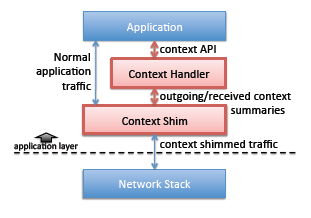
\includegraphics[width=0.4\textwidth]{resources/grapevine_architecture.png}
  \end{center}
\vspace{-20pt}
  \caption{Grapevine System Architecture \cite{grapevine} \label{grapevine_architecture}}
\end{wrapfigure}

As shown in Fig.~\ref{grapevine_architecture}, the {\em Context Handler} computes the context summaries with Bloomier filters to formulate groups based on the group definitions, while the {\em Context Shim} attaches the updated context summary to the outgoing packets and detaches the incoming context summary of the incoming packets, which uses the {\em interceptor} design pattern to work with the {\em Context Handler}. Furthermore, a static notion of $\tau$ is used to address the tradeoff between dissemination cost and the scope of shared context.

\begin{wrapfigure}{r}{0.4\textwidth}
  \begin{center}
    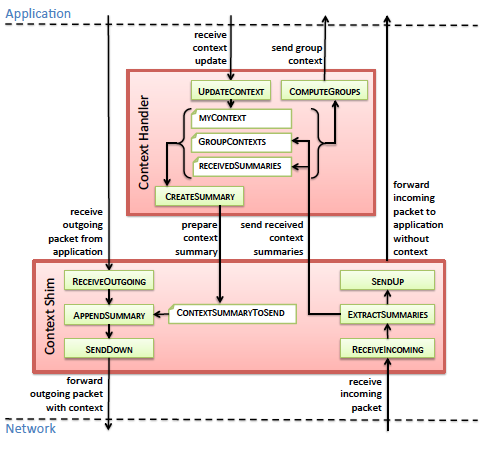
\includegraphics[width=0.4\textwidth]{resources/grapevine_implementation.png}
  \end{center}
  \vspace{-20pt}
  \caption{Information Flow in the Context Shim and Context Handler of Grapevine \cite{grapevine} \label{grapevine_flow}}
    \vspace{-20pt}
\end{wrapfigure}

In implementation, Grapevine uses Java to gain transparency in deployment platform and fine-grained control over the network layer. The information flow of Grapevine, as shown in Fig.~\ref{grapevine_flow}, illustrates how the {\em Context Handler} interacts with the application to compute group membership and context, to store a map of entity context, and to create Bloomier filters for the {\em Context Shim} to access the context summary. The performance and effectiveness of Grapevine are evaluated through a simulated network of 10-by-10 grid and the Pharos multi-robot testbed\cite{agmon2008multi}.


\subsection{Gander}
In contrast to the traditional indexing and ranking methods that require a global view of context connectivity and chronicle archives such as PageRank\cite{page1999pagerank}, the Gander search engine \cite{michel2013gander} provides an IoT perspective to the spatiotemporal queries in the {\em Personalized Networked Spaces} (PNetS). Challenges of searching in the here and now include the privacy and security of personal data, rapidly changing context and conditions, and the impracticality of centrally indexing a constantly growing amount of data. Moreover, by limiting a search within constrained neighborhood and spatiotemporal context, more efficient network and computing resources could be attained.

In order to match the {\em query resolution}, {\em query constraints} and {\em reachability} need to be defined to measure the {\em relevance metric}. Furthermore, a {\em tuple space} is used to provide the {\em global virtual data structure} \cite{picco2002global} distributed in a dynamic network. Since it's impractical to obtain global view in PNetS, query protocols have to be operated within the surrounding data. To find the most relevant query results within a constrained neighborhood of nodes, Gander {\em samples} result candidates in five styles, which are illustrated in Fig.~\ref{gander_sampling}.

\begin{figure}[h]
  \begin{center}
    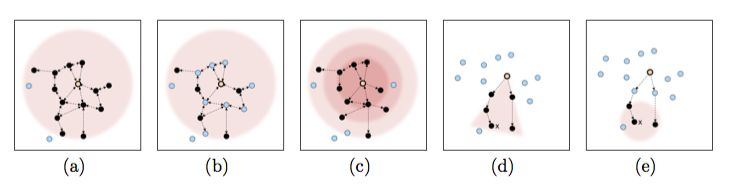
\includegraphics[width=1.0\textwidth]{resources/gander_sampling.png}
  \end{center}
  \vspace{-20pt}
  \caption{Query sampling styles\cite{michel2013gander}. Dashed lines represent sent messages, and darkened nodes are those who respond to a given query. (a) Flooding (b) Random (c) Probabilistic (d) Directional (e) Regional  \label{gander_sampling}}
    \vspace{-10pt}
\end{figure}

Each of the five sampling styles demonstrates the tradeoff between quality and cost in network overhead and latency. {\em Flooding} attempts to reach every node within the network hops, {\em Random} parameterizes the likelihood of responses, {\em Probabilistic} forwards received messages based on a locality probabilistic distribution, {\em Directional} constraints the sampling within a certain heading and angle, and {\em Regional} aims at a given target area. Moreover, a secondary contextual queries are carried out from potential result's perspective, which collects local conditions without adding network overhead and delays.

\begin{wrapfigure}{r}{0.4\textwidth}
\vspace{-20pt}
  \begin{center}
    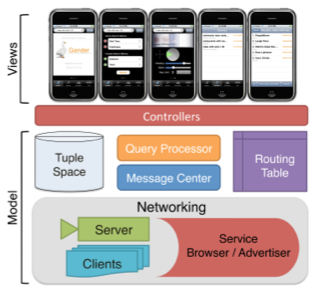
\includegraphics[width=0.4\textwidth]{resources/gander_architecture.png}
  \end{center}
  \vspace{-20pt}
  \caption{{\em myGander} Architecture \cite{michel2013gander} \label{gander_architecture}}
    \vspace{-20pt}
\end{wrapfigure}

The implementation of Gander, {\em myGander}\cite{michel2012mygander}, follows the model-view-controller architecture pattern as shown in Fig.~\ref{gander_architecture}. The model consists of a tuple space implementing the data structure, a routing table that maintains the connectivity in the network, a query processor that handles incoming queries to the tuple space, performs secondary contextual queries on the collected data and meta-data, and routes the results according to its sampling style.

To evaluate sampling protocols in a real world large scale network is extremely challenging. In practice, benchmark simulation for {\em myGander} can be done with OMNet++\cite{varga2001omnet++} for networking and SUMO\cite{krajzewicz2002sumo} for node mobility, in which each node uses its own global virtual data structure to process queries and connects to other mobile node through a proxy.

\subsection{DAIS}

\section{Architecture Design \& Patterns}

\subsection{Gander: The Search of Here and Now}
With the rise of sensor-enhanced objects and computationally-powerful mobile devices, the need for a dynamic search engine that is adaptive to the surrounding spaces and query context is inevitable. 

Gander \cite{michel2012mygander}


	
\section{Current State, Drawbacks, and Future Improvements}

Dynamic network hop $\tau$ in Grapevine.

\Section{Conclusion}

\section*{Acknowledgment}
This paper wouldn't be possible without the advices and feedback provided by Dr. Christine Julien and The Department of Electrical and Computer Engineering at The University of Texas at Austin.

%\medskip
%\noindent

\bibliography{report}
\end{document}

